\begin{figure}[H] \label{img:heliocentrico}
	\centering
	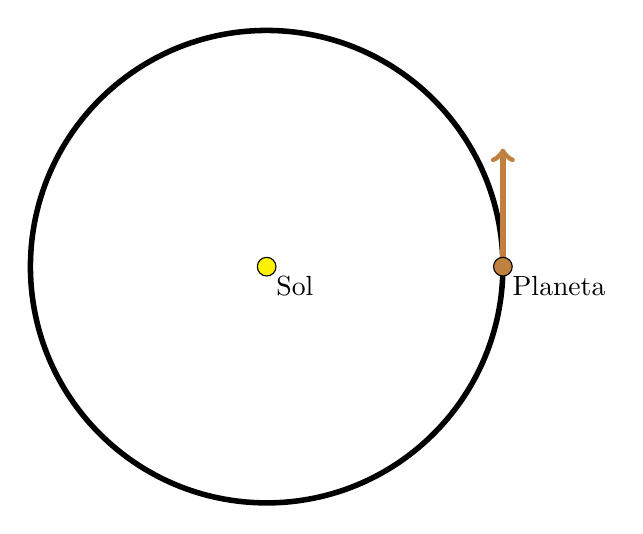
\begin{tikzpicture}[scale=0.75]
	[
		line cap=round,
		line join=round,
		>=triangle 45,
		x=1cm,
		y=1cm
	]
		\draw [line width=2pt] (0,0) circle (4cm);
		\draw [->,line width=2pt,color=brown] (4,0) -- (4,2);
		\draw (0,0) node[anchor=north west] {Sol};
		\draw (4,0) node[anchor=north west] {Planeta};
		\begin{scriptsize}
			\draw [fill=yellow] (0,0) circle (4.5pt);
			\draw [fill=brown] (4,0) circle (4.5pt);
		\end{scriptsize}
	\end{tikzpicture}
	\captionsetup{labelformat=empty}
	\caption{\textbf{Esquema 2:} Modelo heliocêntrico}
\end{figure}